% filepath: /Users/xiangjiahao/tex/weekly_report/2024/12/2024-12-16.tex
\documentclass[11pt,a4paper]{article}
\usepackage{ctex}
\usepackage[utf8]{inputenc}
\usepackage{geometry}
\usepackage{fancyhdr}
\usepackage{enumitem}
\usepackage{titlesec}
\usepackage{amsmath} % Added for math equation support
\usepackage{amssymb}
\usepackage{graphicx} % Added for including graphics
\usepackage{titling}
\usepackage{subcaption}

\usepackage{multicol}
\usepackage{listings}
\usepackage{booktabs}
\usepackage{multirow}

\usepackage[hidelinks]{hyperref}
% \usepackage[style=authoryear]{biblatex} % Use biber backend
% \addbibresource{../../paper.bib} % Specify the .bib file

\geometry{margin=0.5in}
\titleformat{\section}{\large\bfseries}{\thesection}{0.5em}{}

% Title context and style setting
\title{周报-向嘉豪(2024-12-16)}
\setlength{\droptitle}{-6em} % Reduce space before the title
% Redefine \maketitle to display only the title
\renewcommand{\maketitle}{
  \begin{center}
    \LARGE\bfseries\thetitle
  \end{center}
}

\begin{document}

\maketitle

\noindent \textbf{摘要}:
本周,我们对论文进行了深入的修改和完善,主要包括两方面的工作:首先,在参考了\cite{Liu2020}的基础上,我们对论文摘要进行了细分,增加了“动机”和“相关工作”两个小节,以增强摘要的结构性和可读性;其次,我们对实验章节进行了修改,提供了实验测试的开源链接,采用了\cite{Liu2020}中的三线表格样式,深入分析了实验结果,并补充了非SPN结构的密码算法实现。

\noindent \textbf{下周计划}: 1) 完成论文的最终修改和投稿准备;2) 开始准备下一阶段的研究工作。



\subsection{摘要的修改与完善}

在参考了\textit{IEEE Transactions on Computers}中相关文献\cite{Liu2020}后,我们对论文的摘要部分进行了细致的调整。具体而言,我们将摘要细分为多个小节,增加了“动机”和“相关工作”两个部分,以提高摘要的结构性和信息量。在“动机”部分(见图\ref{fig:motivation}),我们详细阐述了研究该问题的重要性和必要性;在“相关工作”部分(见图\ref{fig:related_work}),我们对现有的相关研究进行了系统的综述,明确了本研究的创新点和贡献。

\begin{figure}[h]
  \centering
  \begin{subfigure}[b]{0.3\textwidth}
    \centering
    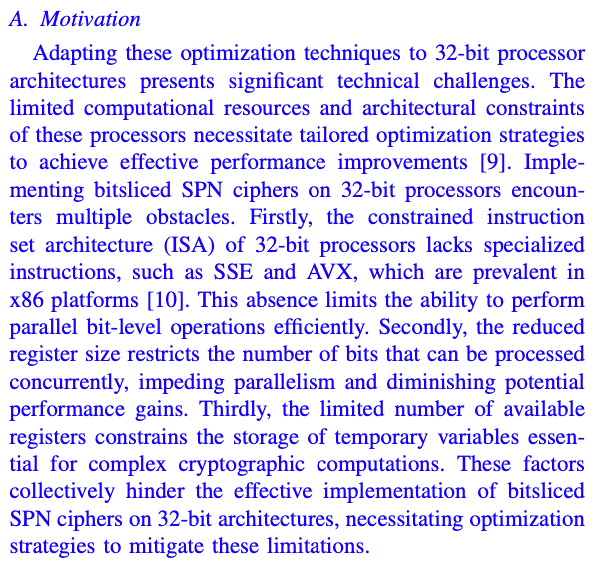
\includegraphics[width=\textwidth]{./fig/motivation.png}
    \caption{动机章节}
    \label{fig:motivation}
  \end{subfigure}
  \hfill
  \begin{subfigure}[b]{0.3\textwidth}
    \centering
    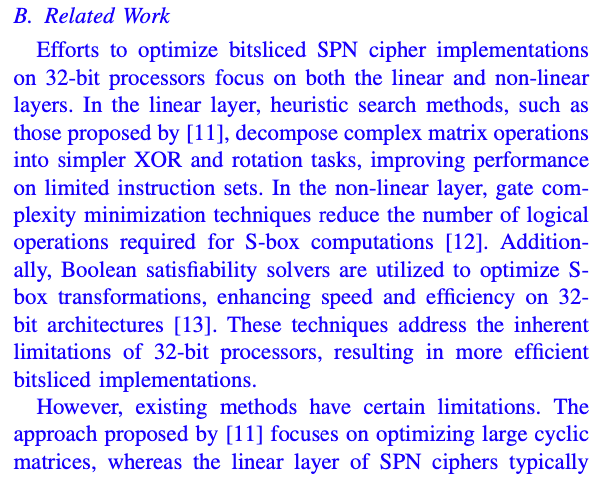
\includegraphics[width=\textwidth]{./fig/relatedWork.png}
    \caption{相关工作章节}
    \label{fig:related_work}
  \end{subfigure}
  \caption{摘要部分的修改}
  \label{fig:combined_figure}
\end{figure}

\subsection{实验章节的改进}

为了提高实验部分的完整性和可重复性,我们提供了实验测试的开源链接。此外,我们将论文中的表格格式由IEEE默认样式改为\cite{Liu2020}中使用的三线表,提高了表格的美观性和规范性。在实验结果分析章节,我们增加了对实验结果的深入讨论和解读(见图\ref{fig:experiment}),以更好地阐释研究成果。为了从更多维度验证我们的方案,我们还补充了非SPN结构的密码算法实现(见图\ref{fig:compare})。

\begin{figure}[h]
  \centering
  \begin{subfigure}[b]{0.3\textwidth}
    \centering
    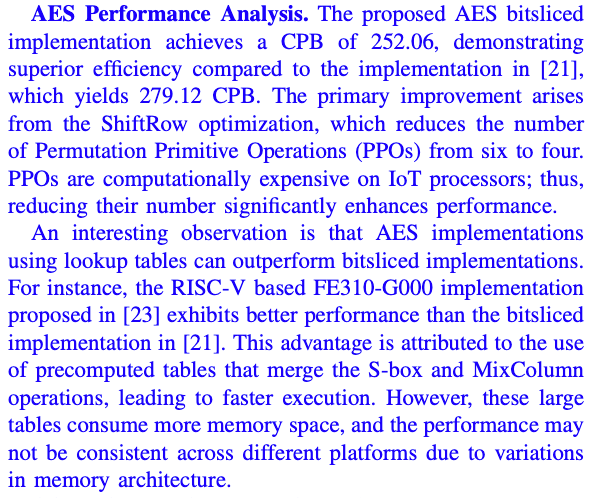
\includegraphics[width=\textwidth]{./fig/aseAnalysis.png}
    \caption{实验结果分析}
    \label{fig:experiment}
  \end{subfigure}
  \hfill
  \begin{subfigure}[b]{0.3\textwidth}
    \centering
    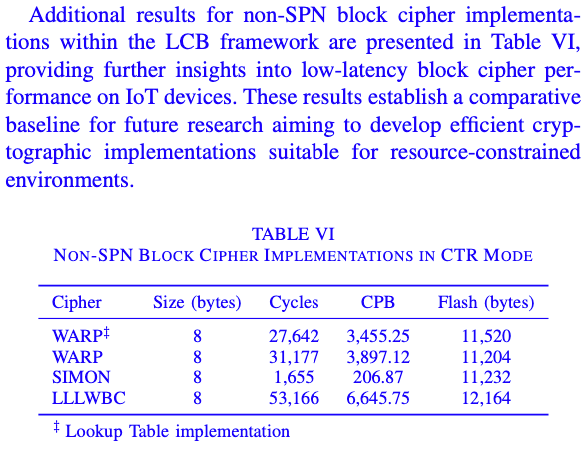
\includegraphics[width=\textwidth]{./fig/nonSPN.png}
    \caption{非SPN结构算法实现}
    \label{fig:compare}
  \end{subfigure}
  \caption{实验章节的改进}
\end{figure}

\newpage

% Include the bibliography
\bibliographystyle{alpha}
\bibliography{../../paper}

\end{document}